% Diagram: KV Cache Growth
\begin{figure}[htbp]
\centering
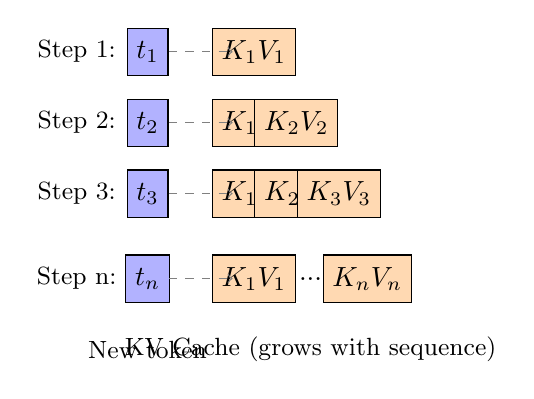
\begin{tikzpicture}[
    scale=0.9,
    cache/.style={rectangle, draw, fill=orange!30, minimum width=0.4cm},
    newtoken/.style={rectangle, draw, fill=blue!30, minimum width=0.4cm, minimum height=0.6cm}
]
% Step 1
\node at (-1, 2) {\small Step 1:};
\node[newtoken] at (0, 2) {$t_1$};
\node[cache, minimum height=0.6cm] at (1.5, 2) {$K_1V_1$};

% Step 2
\node at (-1, 1) {\small Step 2:};
\node[newtoken] at (0, 1) {$t_2$};
\node[cache, minimum height=0.6cm] at (1.5, 1) {$K_1V_1$};
\node[cache, minimum height=0.6cm] at (2.1, 1) {$K_2V_2$};

% Step 3
\node at (-1, 0) {\small Step 3:};
\node[newtoken] at (0, 0) {$t_3$};
\node[cache, minimum height=0.6cm] at (1.5, 0) {$K_1V_1$};
\node[cache, minimum height=0.6cm] at (2.1, 0) {$K_2V_2$};
\node[cache, minimum height=0.6cm] at (2.7, 0) {$K_3V_3$};

% Step n
\node at (-1, -1.2) {\small Step n:};
\node[newtoken] at (0, -1.2) {$t_n$};
\node[cache, minimum height=0.6cm] at (1.5, -1.2) {$K_1V_1$};
\node at (2.3, -1.2) {...};
\node[cache, minimum height=0.6cm] at (3.1, -1.2) {$K_nV_n$};

% Labels
\node at (0, -2.2) {\small New token};
\node at (2.3, -2.2) {\small KV Cache (grows with sequence)};

% Arrows showing cache read
\draw[->, gray, dashed] (0.3, 2) -- (1.2, 2);
\draw[->, gray, dashed] (0.3, 1) -- (1.2, 1);
\draw[->, gray, dashed] (0.3, 0) -- (1.2, 0);
\draw[->, gray, dashed] (0.3, -1.2) -- (1.2, -1.2);

\end{tikzpicture}
\caption{KV cache grows linearly: each new token adds its K/V to the cache and reads all previous entries.}
\label{fig:kv-cache-growth}
\end{figure}
